\section{Braking}

The braking system on the 2010 Formula vehicle is a hydraulically-controlled \emph{disc brake} system. Hydraulic pressure causes callipers on each wheel to squeeze friction pads against the discs, thus braking the vehicle. There are two entirely independent closed hydraulic systems, one for the front brakes and the other for the rear brakes. If one of the systems fails, the other system may be used to safely stop the vehicle. 

The \emph{brake pedal assembly} houses the components used by the driver to engage the brakes, including the \emph{brake pedal}, \emph{brake master cylinders}, and an adjustable \emph{balance bar} for changing the front-rear force distribution. Adjusting the force distribution is called \emph{brake biasing}, and can play a dramatic role in the performance of the vehicle. However, proper brake biasing is a tedious and difficult procedure.

\subsection{Brake Pedal Assembly}

A brake pedal in the cockpit is used to engage the brakes. Two \emph{brake master cylinders} (one for the front system and the other for the rear system) are connected to the brake pedal by way of an adjustable \emph{balance bar}. The balance bar distributes force from the brake pedal to the master cylinders \cite{TiltonBrakeBias}. 

The brake pedal, master cylinders, and balance bar are attached to a modular frame that is located at the end of the cockpit. Together, these components form the \emph{brake pedal assembly}. A model of this assembly is shown in Figs. \ref{fig:brake_pedal_assy_a} and \ref{fig:brake_pedal_assy_b}. Removal of the brake pedal assembly is difficult because the brake lines that connect to the master cylinder cannot be removed without depressurizing both the front and rear brake systems. 

\begin{figure}[h!]
	\centering
		\subfigure[Front view]{
			\label{fig:brake_pedal_assy_a}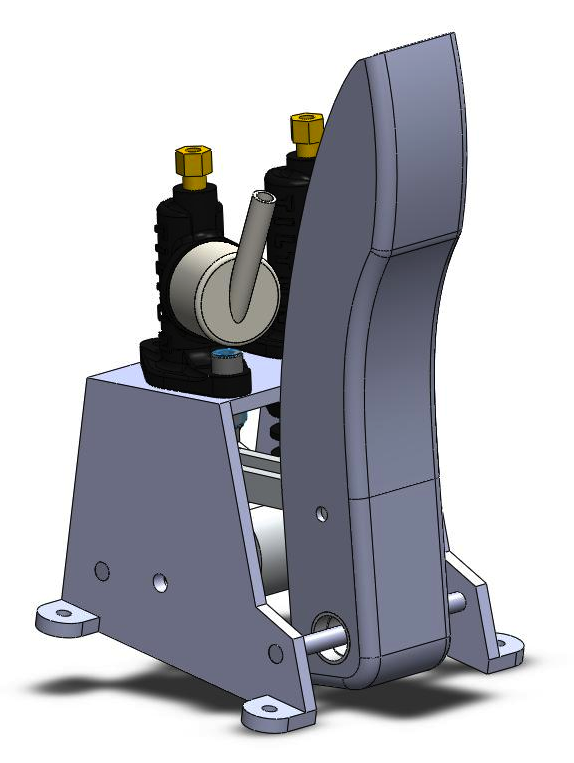
\includegraphics[scale=0.4]{background/figures/brake_pedal_assy_a.eps}}
		\subfigure[Rear view]{
			\label{fig:brake_pedal_assy_b}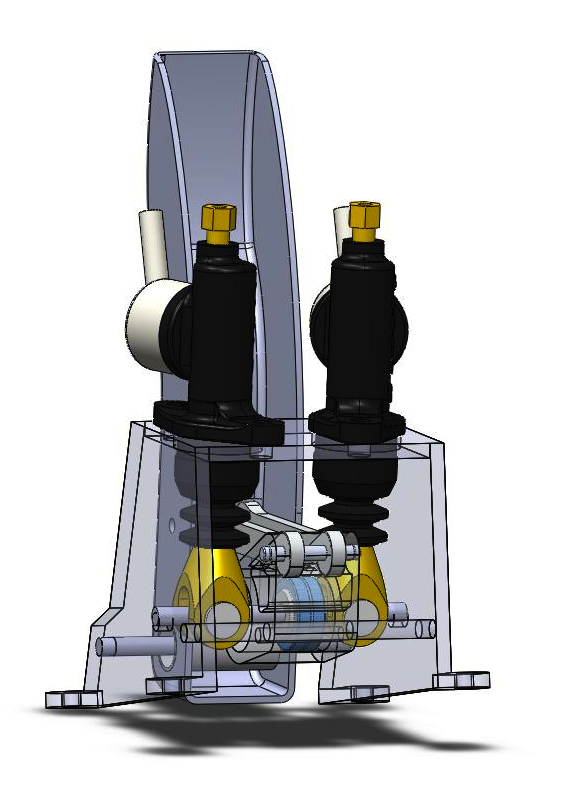
\includegraphics[scale=0.4]{background/figures/brake_pedal_assy_b.eps}}
    \caption{Rendering of the brake pedal assembly.}
    \label{fig:brake_pedal_assy}
\end{figure}

\subsection{Brake Biasing}

Changing the relative braking force between the front and rear is called \emph{brake biasing}. For example, having 65\% of the braking force applied to the front wheels and 35\% to the rear is denoted as "65/35" brake biasing. 

Most of the vehicle weight is in the rear, where the engine is mounted. During braking, weight is effectively transferred from the rear of the vehicle to the front. This weight transfer reduces the braking force available to the rear tires. If too much rear brake force is applied, the rear tires may lock-up and the vehicle will lose traction \cite{FundVehicleDynamics}. This situation can be avoided by properly biasing the brakes for driving conditions.

The relative force provided to each brake master cylinder can be changed by rotating the \emph{balance bar}. When the balance bar is centred between the front and rear cylinders, an equal amount of force will be applied to each. The relationship between the deviation of the adjusting shaft from its centre position and the relative force applied to each cylinder is approximately linear for a range between 70/30 and 30/70 \cite{TiltonBrakeBias}. 

\subsection{Difficulties in Bias Adjustment}

Adjusting the brake bias in virtually all previous generations required removing body panels or the front nose cone, and manually turning a knob on the bias bar. Finding an appropriate setting for brake bias was a tedious trial and error exercise, as drivers had to run a lap in the car, brake heavily, and then return to the team so that the body could be removed and the bias adjusted. Often, drivers were unsatisfied with the bias chosen by another driver, which meant a (likely sub-optimal) compromise in bias point had to be chosen.
